\documentclass[11pt,a4paper]{article}
\usepackage[latin5]{inputenc}
\usepackage[english]{babel}
\usepackage{amsmath}
\usepackage{amsfonts}
\usepackage{amssymb}
\usepackage{graphicx,subfig}
\usepackage{placeins}
\usepackage{gensymb}


\begin{document}

\section{Hough transformation}
\subsection{Step size}
We have compared the results of the Hough transformation while varying different parameters.
For the parameter rho (Fig. \ref{fig:a2b}), we have discovered that making it too large will result in some lines being "overlooked", as the big step sizes simply step over the direction of a line. For theta (Fig. \ref{fig:a2a}), a larger value will discover more lines. This is, because when more finely grained, votes for the same line in the image will be distributed among neighboring accumulator cells, where as when coarsly grained, a single accumulator cell might indicate multiple similar lines. For the number of votes needed to be classified as a line (Fig. \ref{fig:a2c}), we obtained the intuitive result of getting more lines, the less votes are needed.


\begin{figure}%
\centering
\subfloat[][Rho = 0.5\degree]{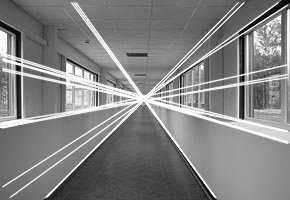
\includegraphics[scale=.3]{hough/res/corridorr0_5.jpg}}
\quad
\subfloat[][Rho = 1.0\degree]{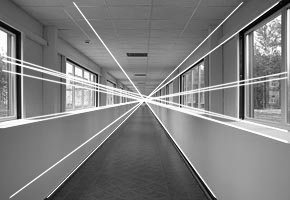
\includegraphics[scale=.3]{hough/res/corridor.jpg}}
\quad
\subfloat[][Rho = 2.0\degree]{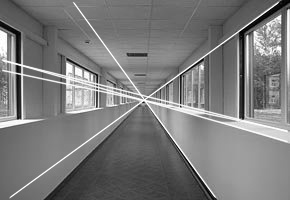
\includegraphics[scale=.3]{hough/res/corridorr2.jpg}}
\quad
\caption{Hough transform for detecting lines with varying rho.}%
\label{fig:a2b}%
\end{figure}

\begin{figure}%
\centering
\subfloat[][Theta = 0.5]{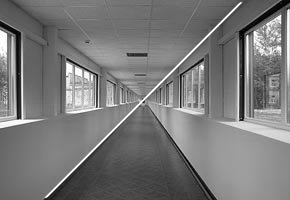
\includegraphics[scale=.3]{hough/res/corridort0_5.jpg}}
\quad
\subfloat[][Theta = 1.0]{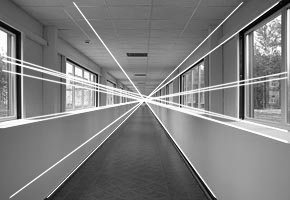
\includegraphics[scale=.3]{hough/res/corridor.jpg}}
\quad
\subfloat[][Theta = 2.0]{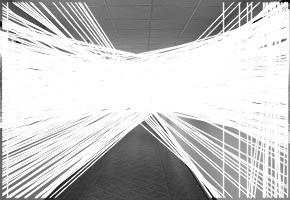
\includegraphics[scale=.3]{hough/res/corridort2.jpg}}
\quad
\caption{Hough transform for detecting lines with varying theta.}%
\label{fig:a2a}%
\end{figure}

\begin{figure}%
\centering
\subfloat[][N = 80]{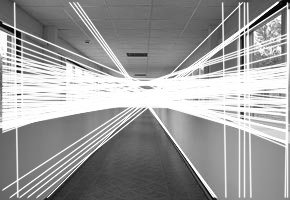
\includegraphics[scale=.3]{hough/res/corridorn80.jpg}}
\quad
\subfloat[][N = 100]{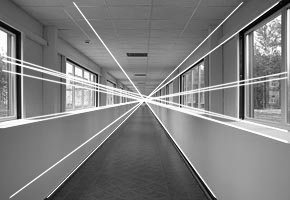
\includegraphics[scale=.3]{hough/res/corridor.jpg}}
\quad
\subfloat[][N = 120]{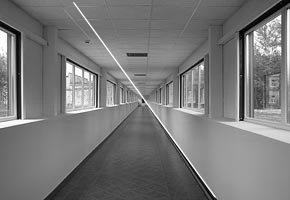
\includegraphics[scale=.3]{hough/res/corridorn120.jpg}}
\quad
\caption{Hough transform for detecting lines with varying number of votes N needed to be classified as line.}%
\label{fig:a2c}%
\end{figure}

\subsection{Line detection}
Here, we have summarized our results in Fig. \ref{fig:a2d} with tuned parameters.

\begin{figure}%
\centering
\subfloat[][theta=1,rho=1\degree,N=100]{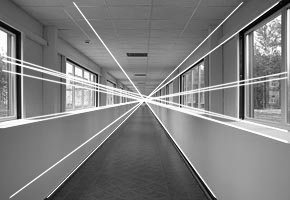
\includegraphics[scale=.3]{hough/res/corridor.jpg}}
\quad
\subfloat[][theta=3/4,rho=3/4\degree,N=140]{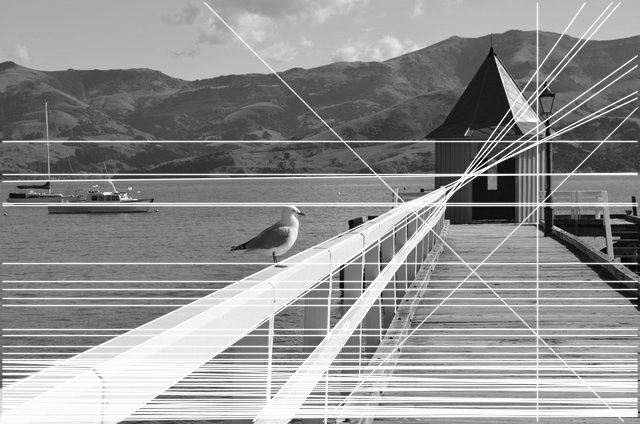
\includegraphics[scale=.3]{hough/res/outdoor.jpg}}
\quad
\subfloat[][theta=3/4,rho=3/4\degree,N=77]{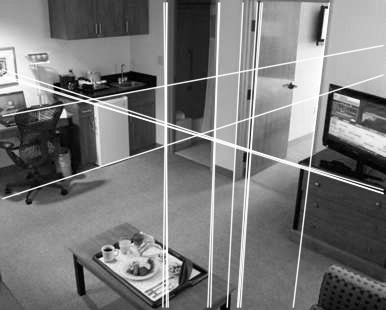
\includegraphics[scale=.3]{hough/res/room_1.jpg}}
\quad
\subfloat[][theta=3/4,rho=3/4\degree,N=105]{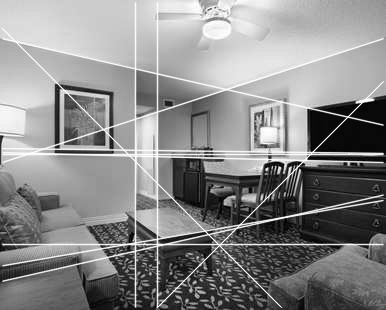
\includegraphics[scale=.3]{hough/res/room_2.jpg}}
\quad
\subfloat[][theta=1,rho=1\degree,N=130]{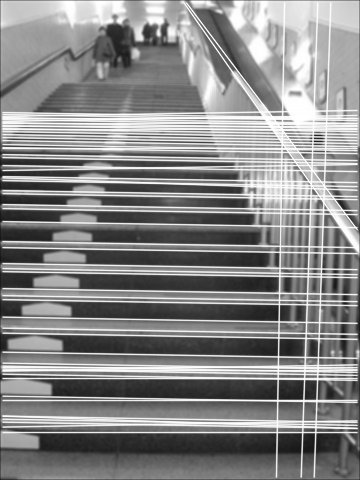
\includegraphics[scale=.3]{hough/res/stairs.png}}
\quad
\caption{Line detection with Hough, preprocessed with Canny}%
\label{fig:a2d}%
\end{figure}

\subsection{Complexity}
Since the algorithm has to test for every combination of rho and theta, the complexity is proportional to the number of rhos times the number of thetas.

\subsection{Multiple lines detected}
Our approach to solving the propblem of multiple similar lines being detected for the same line in the image is a rather simple one. Since these similar lines lie closely together in the hough accumulator (mostly neighboring cells), we need a way to combine clusters of high valued cells. We would do this by blurring the image, for example by convolving with a gauss kernel and then either apply a threshold function to the accumulator or subsample the accumulator to halve it in size. Repetition of this should eliminate the double-detection of the same lines.

\subsection{HoughLinesP}
We have tried out the HoughLinesP function with the same parameters as above, except that we adjusted the number of votes needed to 1/3rd of the above numbers. We have discovered that this function is better at finding also short lines. The results can be seen in Fig. \ref{fig:a2e}

\begin{figure}%
\centering
\subfloat[][theta=1,rho=1\degree,N=33]{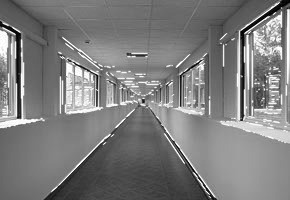
\includegraphics[scale=.3]{hough/res/Pcorridor.jpg}}
\quad
\subfloat[][theta=3/4,rho=3/4\degree,N=46]{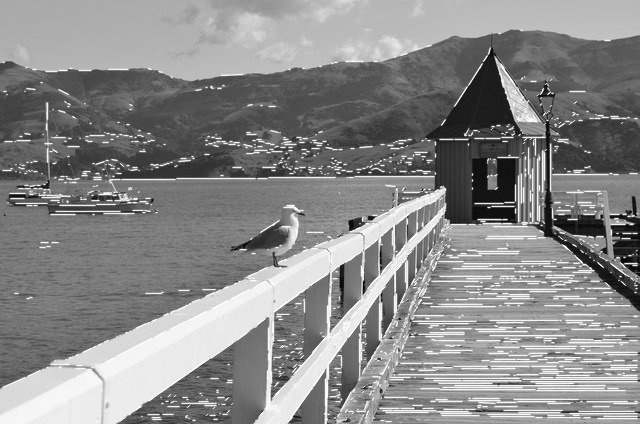
\includegraphics[scale=.3]{hough/res/Poutdoor.jpg}}
\quad
\subfloat[][theta=3/4,rho=3/4\degree,N=25]{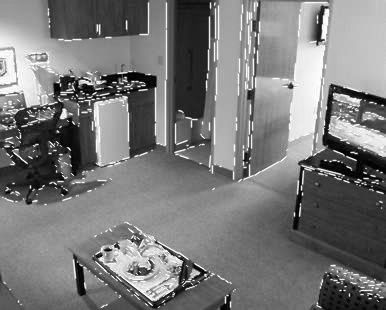
\includegraphics[scale=.3]{hough/res/Proom_1.jpg}}
\quad
\subfloat[][theta=3/4,rho=3/4\degree,N=35]{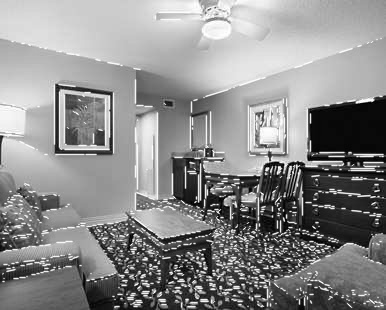
\includegraphics[scale=.3]{hough/res/Proom_2.jpg}}
\quad
\subfloat[][theta=1,rho=1\degree,N=43]{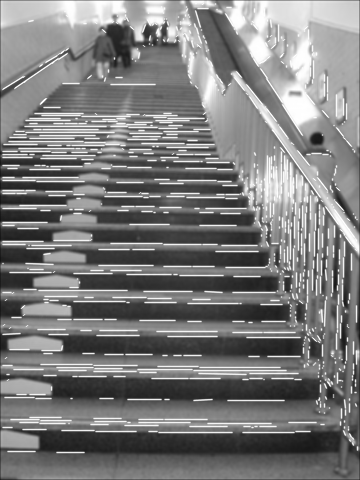
\includegraphics[scale=.3]{hough/res/Pstairs.png}}
\quad
\caption{Line detection with HoughLinesP, preprocessed with Canny}%
\label{fig:a2e}%
\end{figure}

\end{document}
